\newpage
\section{Literature Review}
\subsection{Business Review / Software Review}
\subsubsection*{Calendly}
\begin{center}
    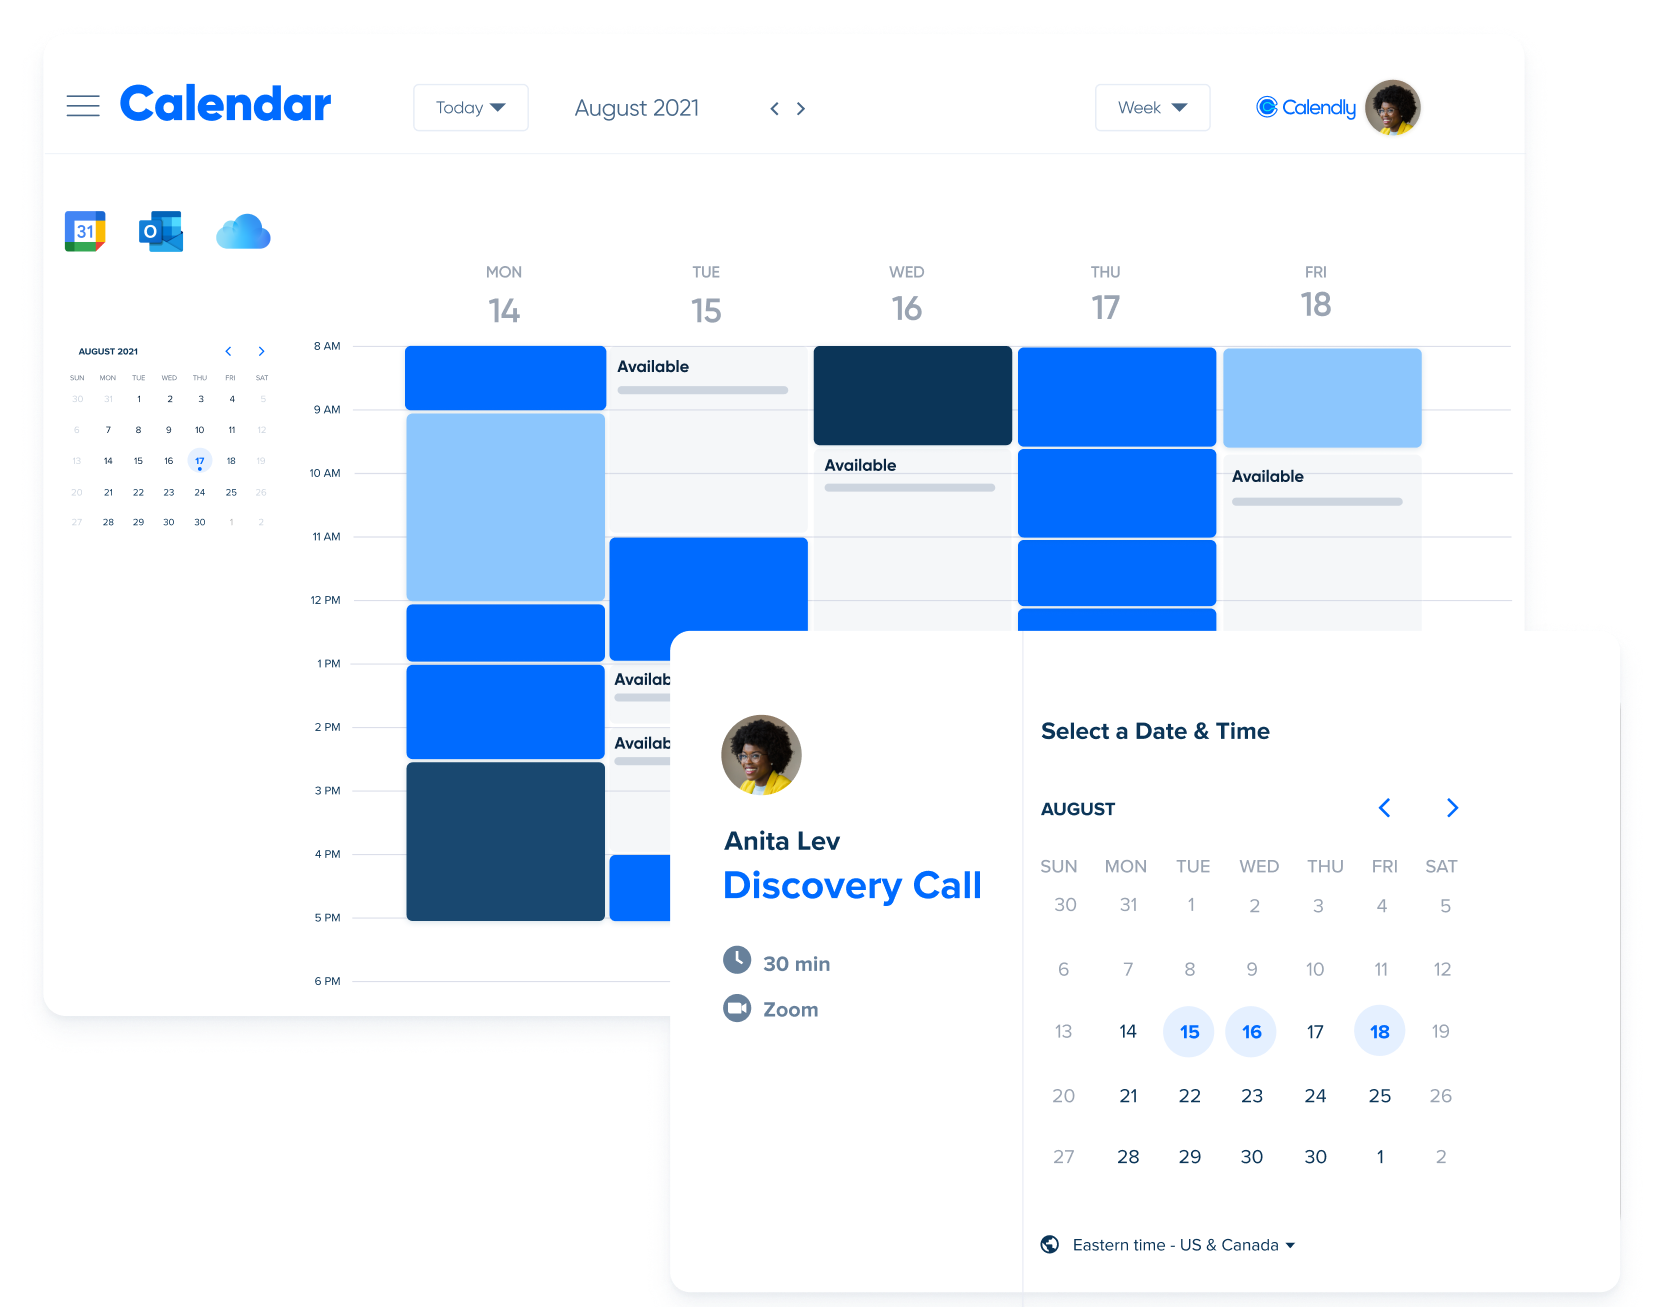
\includegraphics[width=0.7\textwidth]{images/CalendarConnections.png}
\end{center}
\textbf{Calendly}\cite{calendly_ref} is an automated scheduling platform that eliminates back-and-forth emails by allowing users to share their availability links, enabling invitees to instantly book open time slots.
\subsubsection*{Savvycal}
\begin{center}
    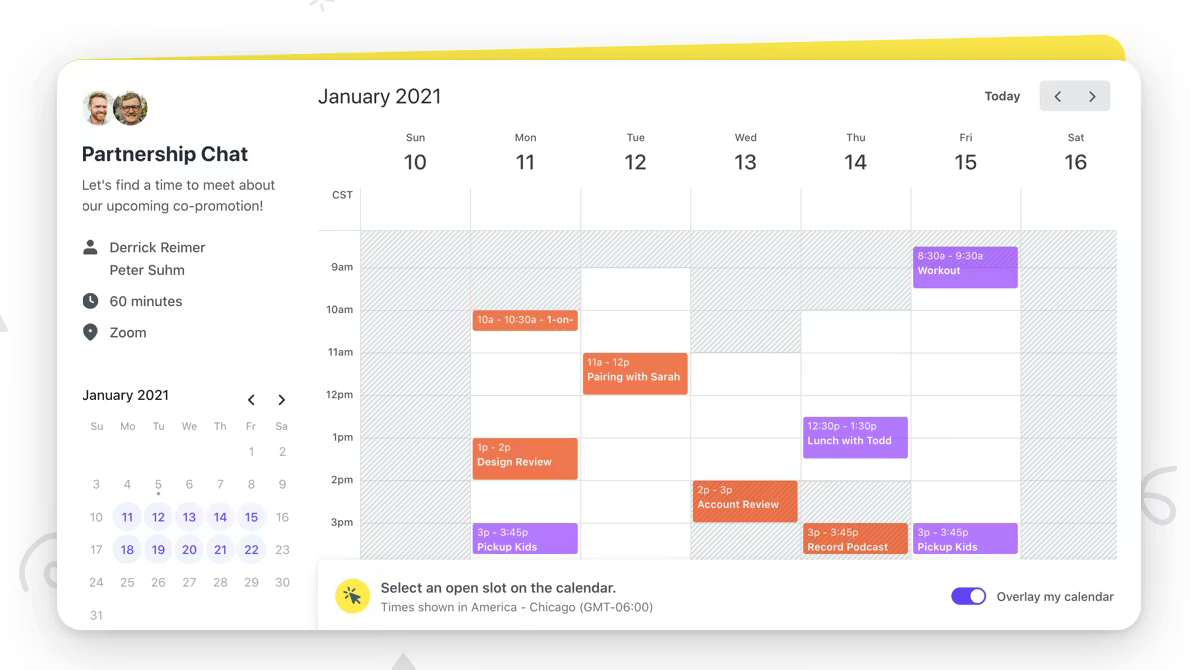
\includegraphics[width=0.7\textwidth]{images/Savvycall.png}
\end{center}
\textbf{Savvycal}\cite{savvycal_ref} is a collaborative scheduling tool featuring an interactive calendar overlay, which allows recipients to lay their own calendar over the sender's schedule to easily find mutual availability.
\subsubsection*{Doodle}
\begin{center}
    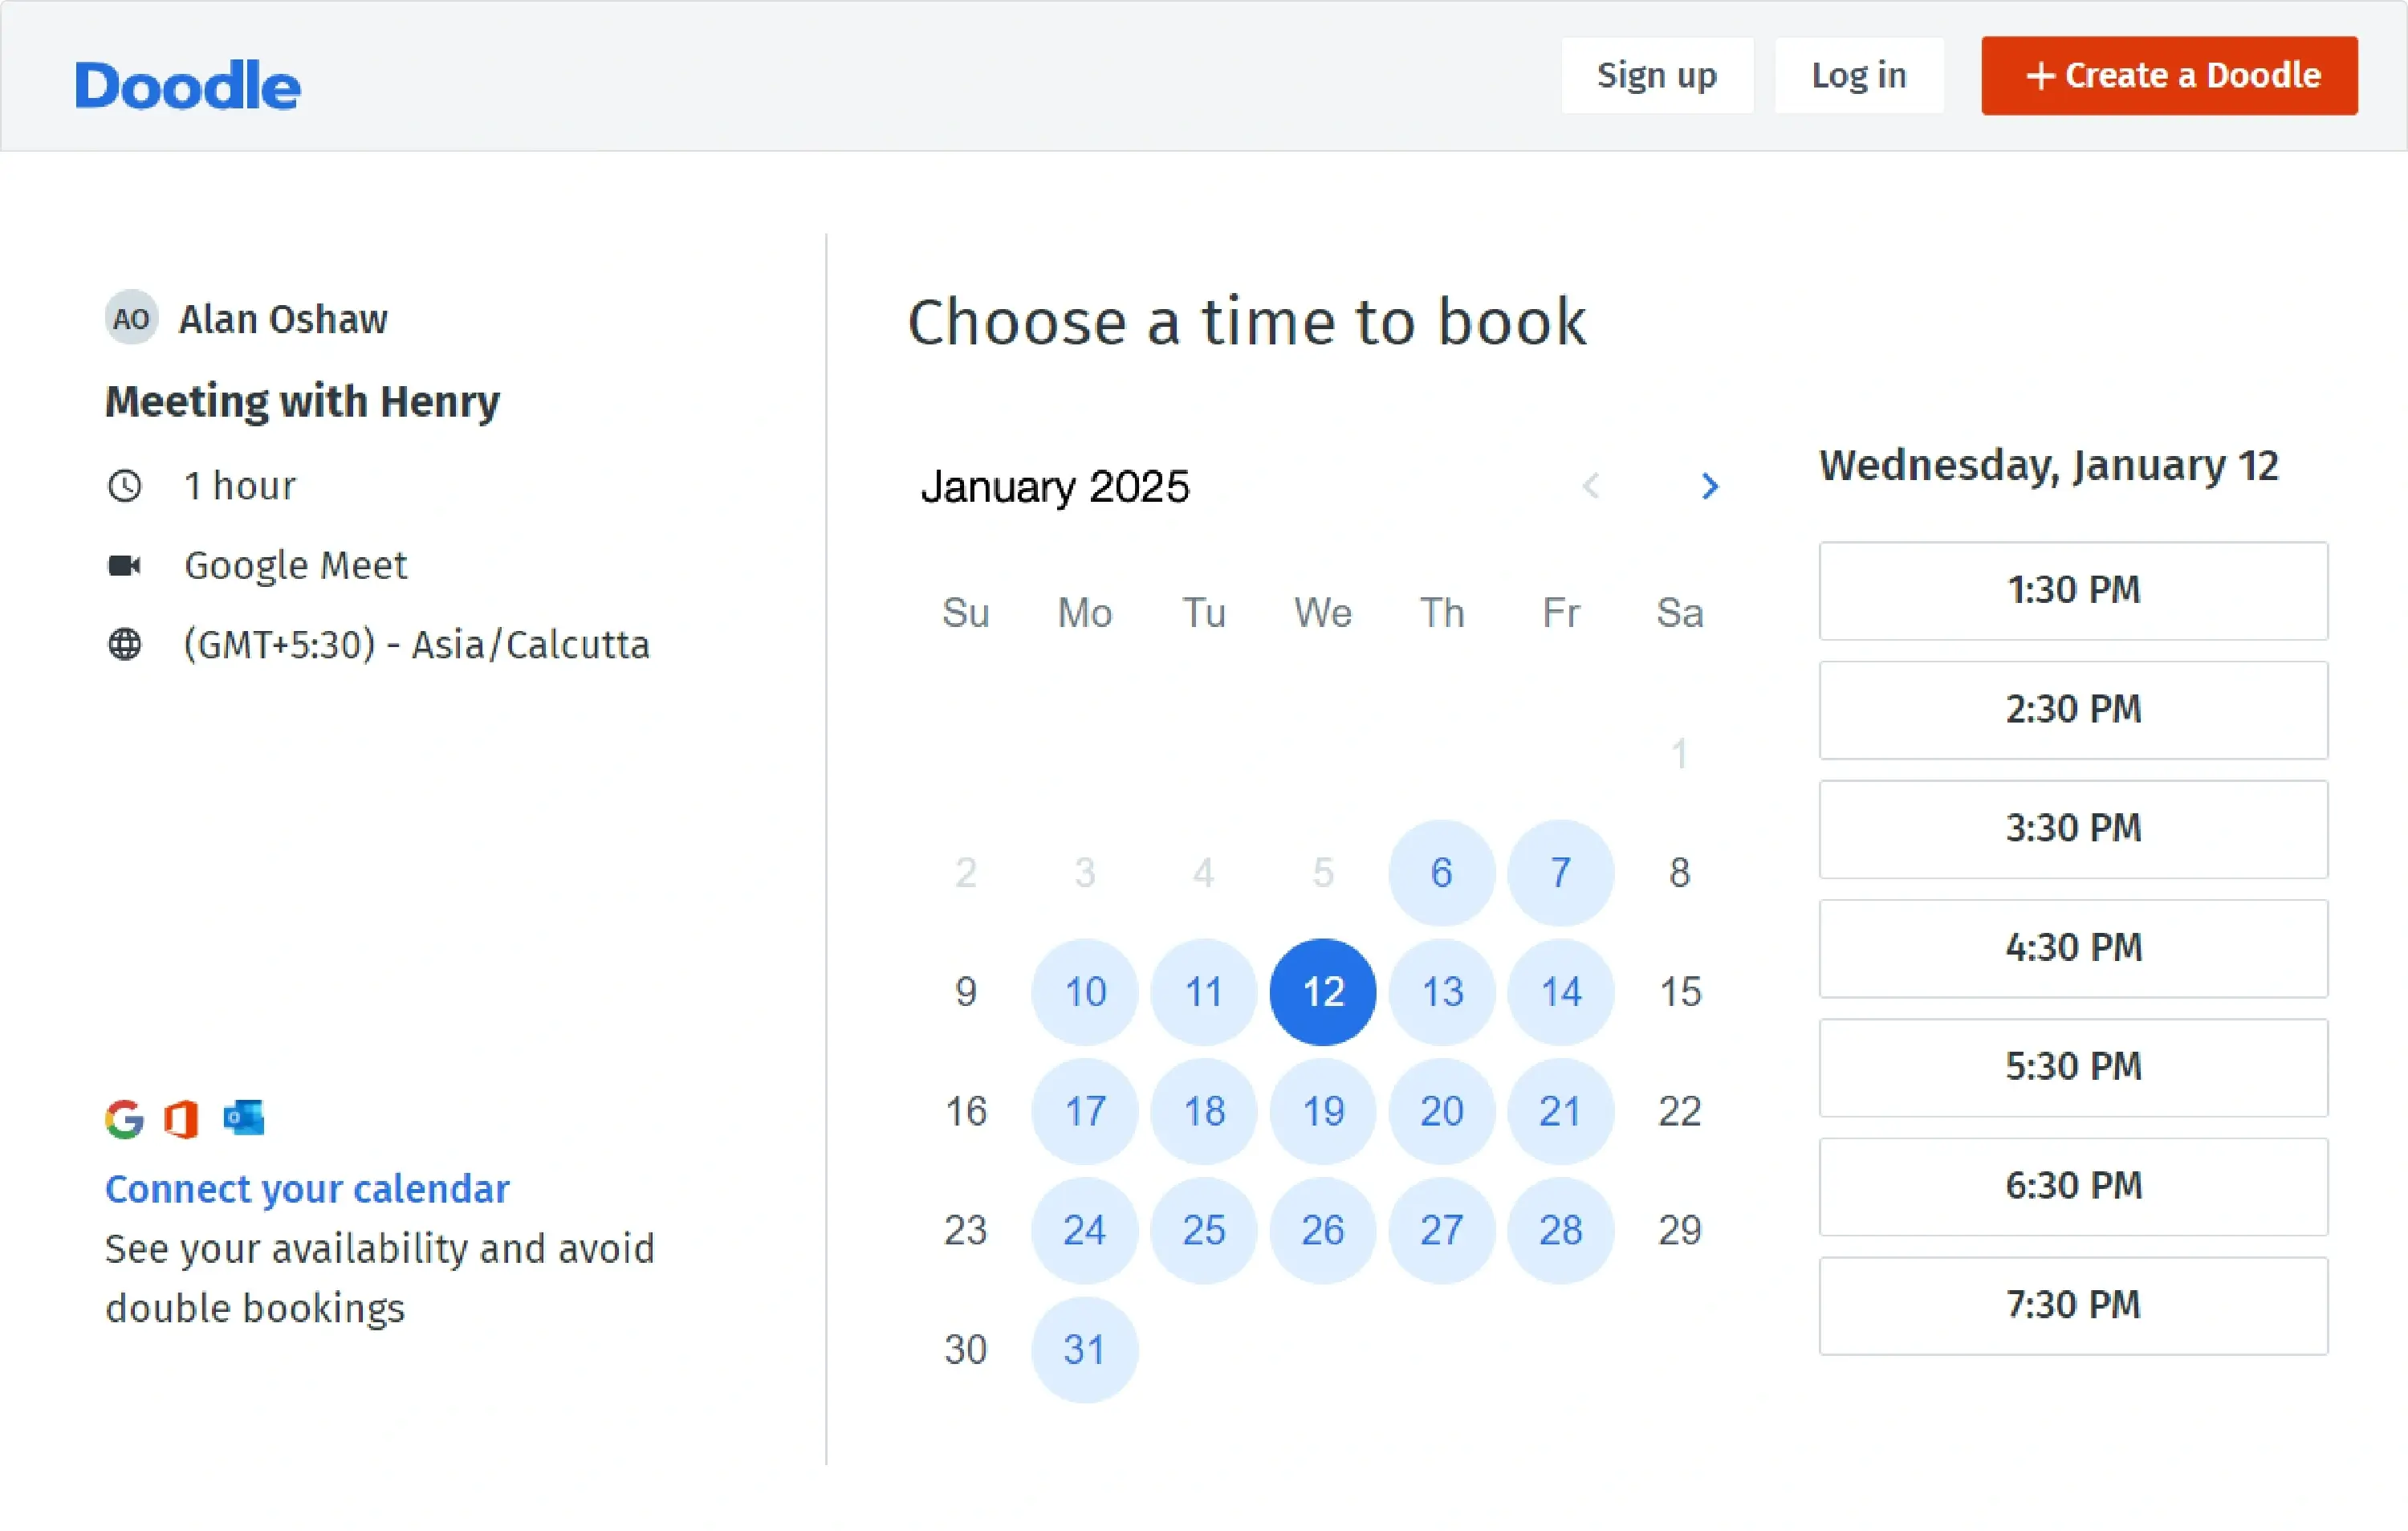
\includegraphics[width=0.7\textwidth]{images/doodle-img.png}
\end{center}
\textbf{Doodle}\cite{doodle_ref} is a group scheduling platform that utilizes a polling system, where an organizer proposes multiple time options and participants vote on their availability to determine the best consensus time for a meeting.

\subsubsection*{Comparative Table}
\vspace{0.5 cm}
\mytable{|X[1.5,l]|X[l]|X[l]|X[l]|X[1.5,l]|X[0.75,l]|}{
Feature & Calendly & Savvycal & Doodle & Converge \\

Smart Booking System & Partial — Link-Based  & Partial — Overlay-Based  & Partial — Consensus-Based  & Auto-Pick \\

Commute-Aware Scheduling & Partial — Fixed Buffers & Partial — Fixed Buffers & No — Not Supported & Dynamic Buffers \\

Automatic Room Management & Partial — Text-Only  & No — Not Supported  & No — Not Supported  & Auto-allocates  \\

Centralized Schedule Dashboard & NO — User-Centric & No — User-Centric & No — Event-Centric & Business - Centric \\
}

\newpage
\subsection{Architectural Foundations \& Prior Art}
Because generic SaaS tools fail to process spatial-temporal routing and multi-variable constraints, Converge abandons standard scheduling APIs. Instead, the system architecture is built upon established Operations Research and Artificial Intelligence methodologies to solve these specific logistical bottlenecks.
\subsubsection{Constraint Satisfaction Modeling for NP-Hard Problems}
Scheduling a distributed workforce across multiple physical locations is formally classified in computer science as an NP-hard optimization problem. If a standard brute-force algorithm attempts to examine every possible schedule combination, the time required to find a solution rises exponentially, leading to system failure at an enterprise scale.

To resolve this, the Converge core scheduling engine is modeled directly on Constraint Logic Programming (CLP) methodologies\cite{elsakka2015}. By formulating the tutoring schedule as a formal Constraint Satisfaction Problem (CSP), the architecture mathematically isolates hard constraints from soft constraints. The AI engine enforces strict physical realities such as ensuring an instructor is required only once at any given time point, and verifying that physical room occupancy does not exceed capacity before a schedule can be validated. This constraint-based approach guarantees mathematically conflict-free resource allocation without exhausting server memory.
\subsubsection{Spatial-Temporal Routing Constraints}
Generic SaaS scheduling applications are fundamentally ignorant of physical geography, relying entirely on simple temporal time-blocking. However, experience within the timetabling research community dictates that every single institution has its own unique rules, conventions, and operational fixations, rendering off-the-shelf software insufficient for specialized educational logistics\cite{ceschia2022}.

A critical requirement of the Converge architecture is the dynamic dispatching of personnel between physical branches. Addressing this requires a "rich formulation" that incorporates spatial-temporal routing constraints. As highlighted by recent state-of-the-art international timetabling benchmarks, such as the ITC-2019 dataset \cite{ceschia2022}, processing dynamic inter-branch travel times is a hallmark of complex real-world scheduling. Converge implements these findings by utilizing a customizable, pre-configured travel time matrix. By calculating commute buffers based on admin-defined durations between the instructor's previous and upcoming branches, the system instantly prunes invalid paths from the combinatorial search space to prevent impossible transit requirements.
\subsubsection{Heuristic Search and Interactive Explainable AI (XAI)}
When exact matches for student requests fail due to spatial-temporal or resource limitations, the system must calculate optimized alternatives. Because the search space is massive, the architecture implements Heuristic Search methodologies to rapidly score and return the next highest-scoring schedule vectors\cite{schaerf1999}.

Furthermore, fully automated "push-button" timetabling systems often fail in practice because human administrators require the flexibility to negotiate soft constraints directly with clients. Therefore, following Schaerf's findings on automated timetabling\cite{schaerf1999}, Converge is designed as an Interactive Decision Support System. The Symbolic AI engine processes the heavy spatial-temporal mathematics and exposes its logical trade-offs to the frontend via an Explainable AI (XAI) decision trace. This interactive architecture empowers administrative staff to manually finalize sales-driven booking decisions while relying on the backend engine to strictly enforce physical routing and capacity boundaries.

\subsection{Tool and Technology Review}
\subsubsection{Frontend Language}
\noindent
\begin{minipage}{0.15\textwidth}
    \centering
    
\includegraphics[width=1\linewidth]{images/TypeScript.png}
\end{minipage}
\hfill
\begin{minipage}{0.82\textwidth}
We chose \textbf{TypeScript}\cite{typescript_ref} over JavaScript as the frontend language because its compile-time error checking prevents structural logic failures in our multi-branch scheduling. In making this choice, we accept the tradeoff of a slower initial prototyping phase due to strict type definition requirements.
\end{minipage}
\vspace{0.5cm}\\
\mytable{|X[0.6,l]|X[l]|X[l]|X[l]}{
{Aspect / \\ Language} & TypeScript & JavaScript & Dart\\

Typing System & Static Typing & Dynamic Typing & Static Typing\\

Data Structure & Explicit Contracts & Flexible Objects & Classed Based Model\\

Development Tooling &
Strong IDE support &
Basic inference &
Strong Tooling\\

Trade Off &
High strictness overhead &
Risk of runtime errors &
Smaller Web Ecosystem \\
}

\subsubsection{Frontend Framework}
\noindent
\begin{minipage}{0.15\textwidth}
    \centering
    
\includegraphics[width=1\linewidth]{images/Vue.js.png}
\end{minipage}
\hfill
\begin{minipage}{0.82\textwidth}
We chose \textbf{VueJS}\cite{vuejs_ref} over React because its lower learning curve and built-in tooling allow us to focus on building features rather than configuring the project. In making this choice, we accept the tradeoff of a smaller ecosystem.
\end{minipage}
\vspace{0.5cm} \\
\mytable{|X[0.6,l]|X[l]|X[l]|X[l]|}{
{Aspect / \\ Framework} & VueJS & ReactJS & Angular \\

Component Structure &
Single File Component &
JSX &
Component + Template \\

State Management& 
Proxy-based &
Hooks &
Services + RxJS \\

Ecosystem & 
Small ecosystem (official tools) &
Massive ecosystem &
Large enterprise ecosystem \\

Trade Off &
Smaller community &
Steep learning curve &
Heavy framework, verbose \\
}

\newpage
\subsubsection{Backend Language}
\noindent
\begin{minipage}{0.15\textwidth}
    \centering
    \includegraphics[width=1\linewidth]{images/go.png}
\end{minipage}
\hfill
\begin{minipage}{0.82\textwidth}
We chose \textbf{Golang}\cite{golang_ref} over Java and NodeJS as the backend language because its compiled performance and native concurrency model perfectly balance raw execution speed with a low memory footprint. In making this choice, we accept the tradeoff of Go’s verbose syntax and manual error handling, which requires writing more boilerplate code than Node.js.
\end{minipage}
\vspace{0.5cm} \\
\mytable{|X[0.6,l]|X[l]|X[l]|X[l]|}{
{Aspect / \\ Language} & Golang & Java & NodeJS \\

Concurrency Model &
Native &
Thread-Based &
Single-Threaded \\

Execution Model &
Native Binary &
JVM Bytecode &
JIT Interpreted \\

Architecture &
Minimalist \& Explicit &
Strict OOP &
Highly Dynamic \\

Trade Off &
Verbose syntax &
High memory usage &
Potential bottlenecks \\
}

\subsubsection{Backend Framework}
\noindent
\begin{minipage}{0.15\textwidth}
    \centering
    
\includegraphics[width=1\linewidth]{images/gin.png}
\end{minipage}
\hfill
\begin{minipage}{0.82\textwidth}
We chose the \textbf{Gin}\cite{gin_ref} framework over Go’s native standard library (\texttt{net/http}) because its built-in routing and middleware capabilities significantly accelerate the development of our REST API. In making this choice, we accept the tradeoffs of framework lock-in and a slight memory overhead.
\end{minipage}
\vspace{0.5cm} \\
\mytable{|X[0.6,l]|X[l]|X[l]|X[l]|}{
{Aspect / \\ Framework} & Gin & net/http & Fiber \\

Routing &
Advanced &
Basic &
Express-style, fast \\

Middleware Management &
Built-in &
Manual &
Built-in \\

Data Binding \& Validation &
Automated &
Manual &
Limited \\

Ecosystem & 
Mature &
Minimal &
Growing \\

Trade Off &
Slight overhead \& lock-in &
More boilerplate &
Less standard, smaller ecosystem \\
}

\newpage
\subsubsection{Database}
\noindent
\begin{minipage}{0.15\textwidth}
    \centering
    
\includegraphics[width=1\linewidth]{images/PostgresSQL.png}
\end{minipage}
\hfill
\begin{minipage}{0.82\textwidth}
We chose \textbf{PostgreSQL}\cite{postgresql_ref} as the database because its native support for range data types is perfectly suited for a scheduling system. In making this choice, we accept the tradeoff of a steeper learning curve and slightly more configuration overhead.
\vspace{0.5cm} \\
\end{minipage}
\mytable{|X[0.6,l]|X[l]|X[l]|X[l]|}{
{Aspect / \\ Database} & PostgreSQL & MySQL & MongoDB \\

Data Model &
Relational &
Relational &
Document \\

Querying Complex Data &
Advanced &
Standard &
Aggregation-heavy \\

Data Type Support &
Range Types &
Basic Types &
Flexible Documents \\

Trade Off &
Steeper learning curve &
Limited advanced types &
Risk of inconsistency \\
}

\subsubsection{Architectural Pattern}
\noindent
\begin{minipage}{0.15\textwidth}
    \centering
    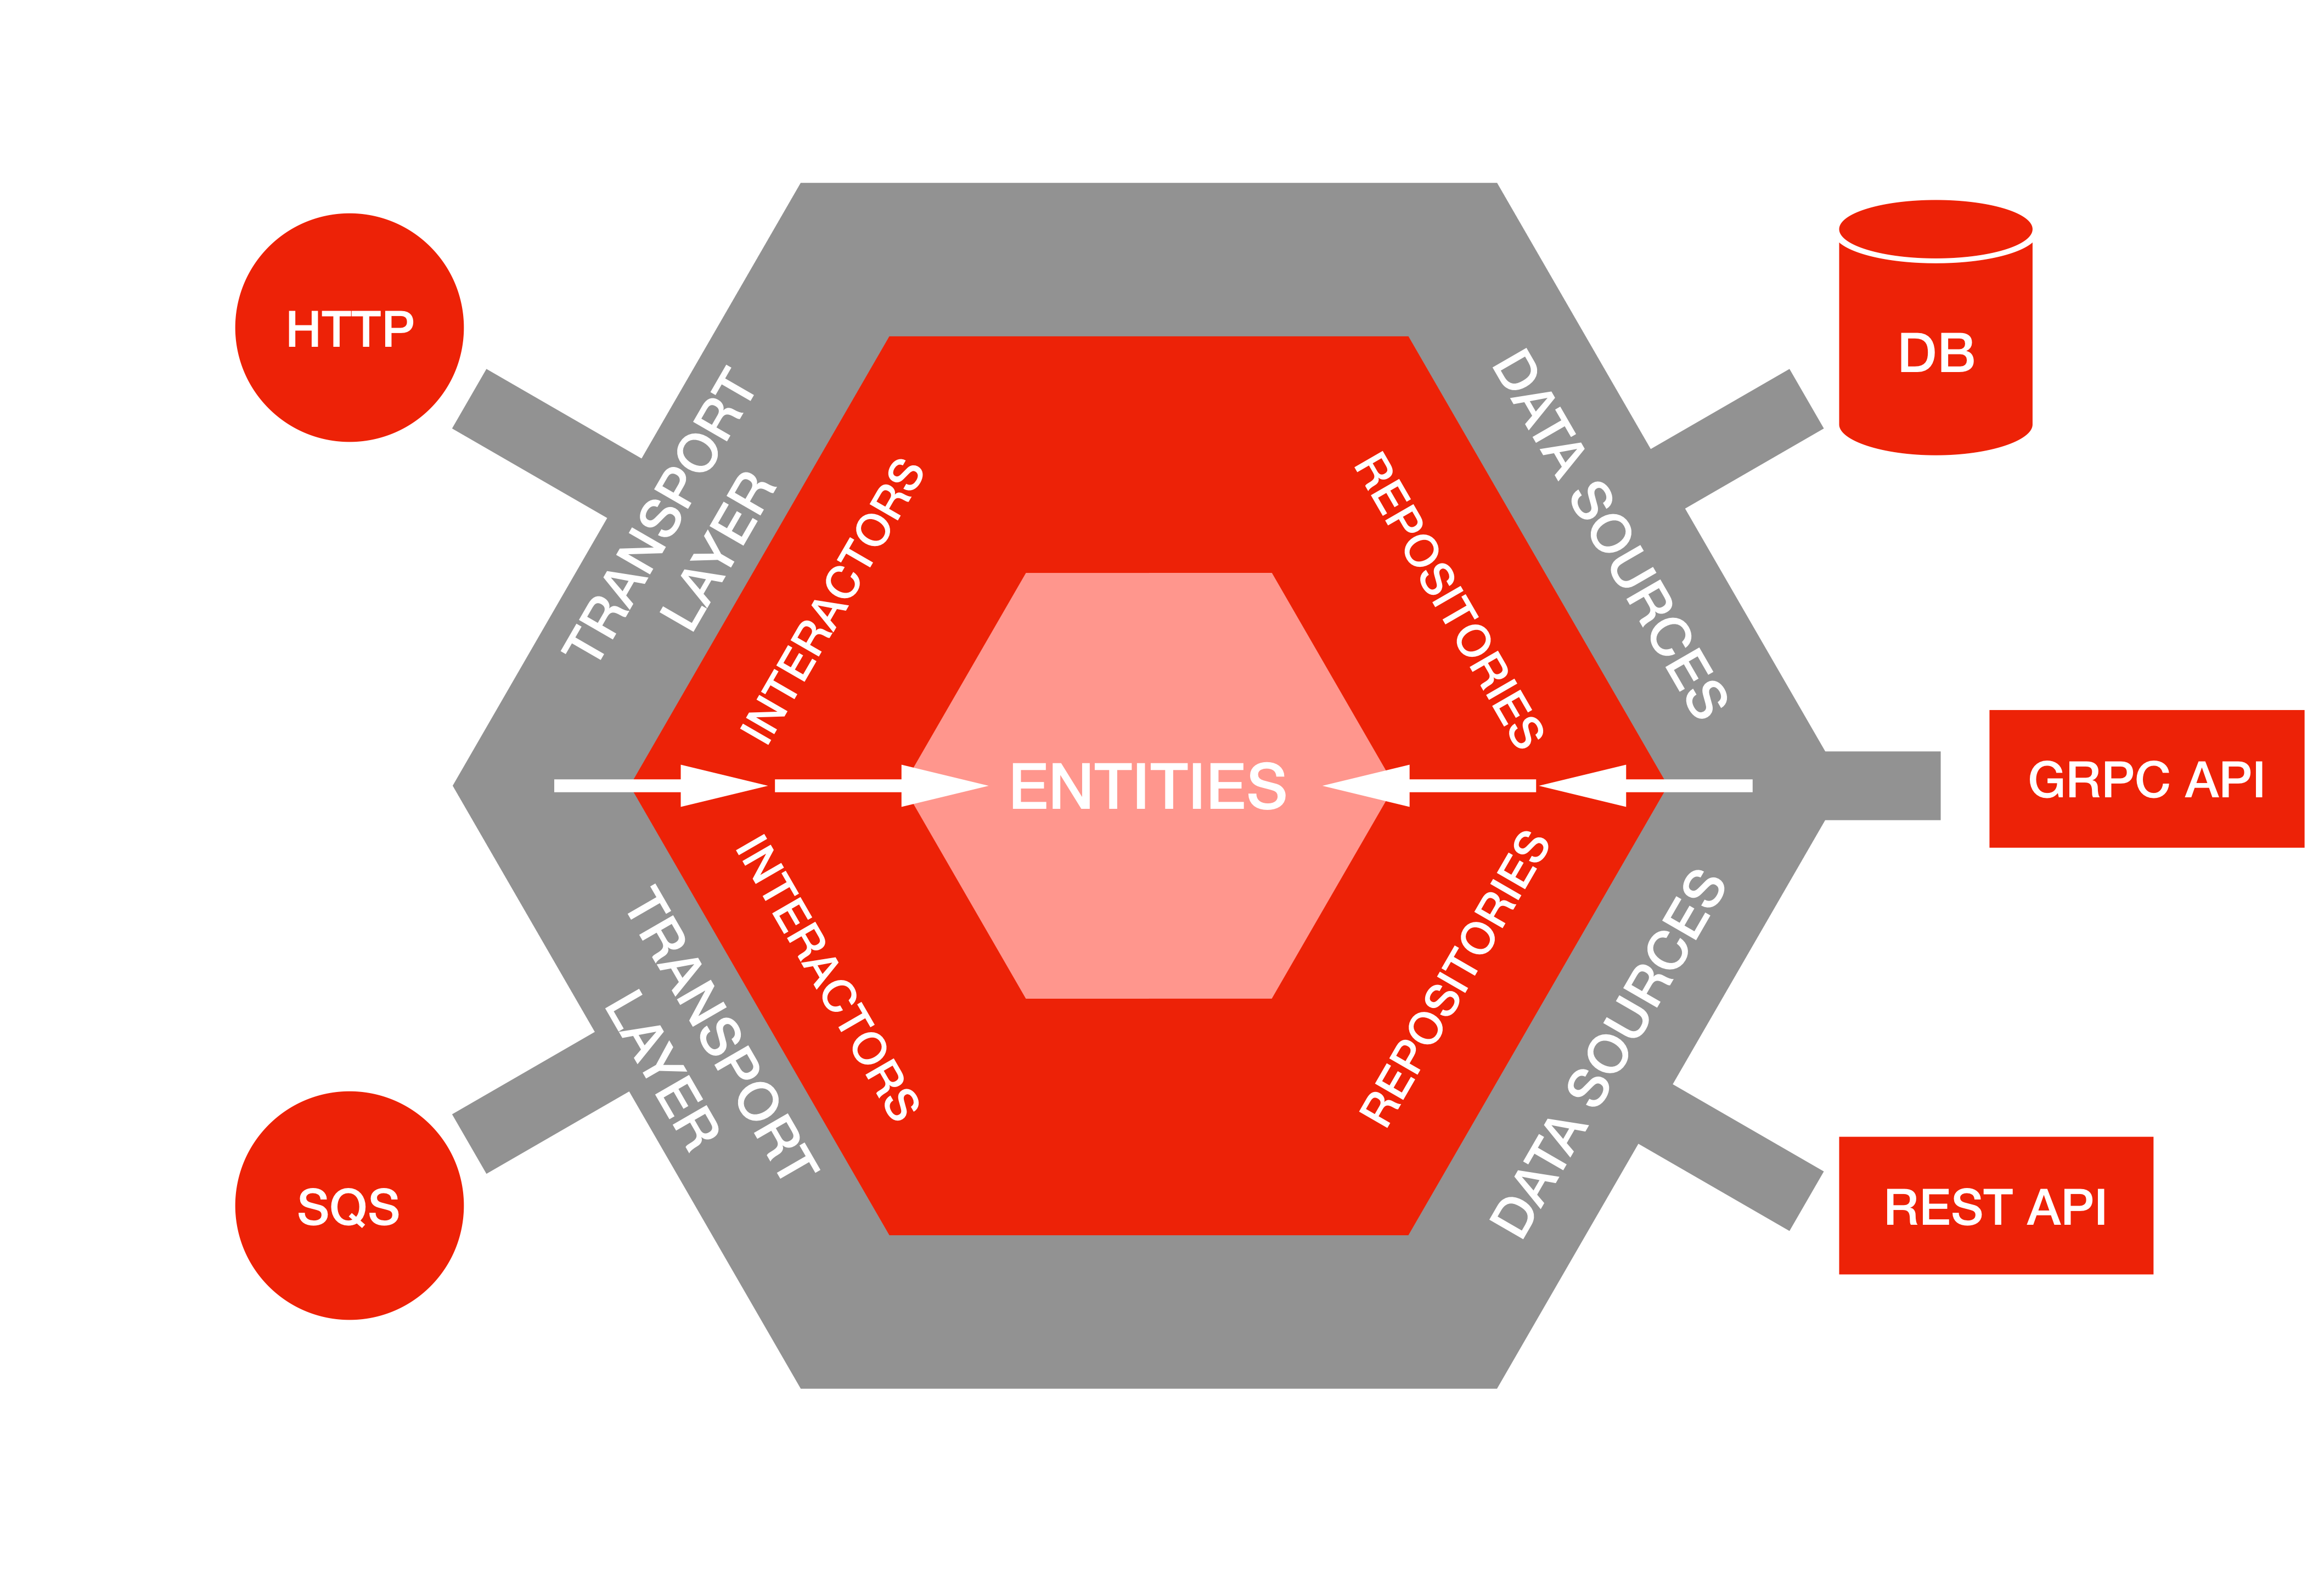
\includegraphics[width=1\linewidth]{images/hexagonal.png}
\end{minipage}
\hfill
\begin{minipage}{0.82\textwidth}
We chose \textbf{Hexagonal Architecture}\cite{hexagonal_ref} as the backend architectural pattern because it keeps the core scheduling domain portable and testable in isolation from the web framework. In making this choice, we accept the tradeoff of increased initial complexity, requiring more folders and interfaces upfront.
\end{minipage}
\vspace{0.5cm} \\
\mytable{|X[0.6,l]|X[l]|X[l]|X[l]|}{
{Aspect / \\ Architect} & Modular Monolith & Microservice & SOA \\

System Complexity &
Moderate &
High &
Moderate–High \\

Domain Modeling &
Well-structured &
Distributed &
Service-based \\

Operational Overhead &
Low &
High &
Moderate \\

Deployment &
Single deployable unit &
Independently deployable services &
Multiple services \\

Trade Off &
Requires discipline &
High infrastructure cost &
Less flexible than microservices, shared dependencies \\
}

\newpage
\subsubsection{Deployment Architecture}
\noindent
\begin{minipage}{0.15\textwidth}
    \centering
    
\includegraphics[width=1\linewidth]{images/modular_monolith.png}
\end{minipage}
\hfill
\begin{minipage}{0.82\textwidth}
We chose a \textbf{Modular Monolith}\cite{architecture_ref} over both Microservices and a standard Monolith to provide a safe evolution path for the system. This approach allows us to properly model the system using Domain-Driven Design (DDD) principles without the immediate operational complexity of a distributed network. In making this choice, we accept the tradeoff of relying on strict developer code discipline to enforce module boundaries, rather than relying on physical infrastructure separation.
\end{minipage}
\vspace{0.5cm} \\
\mytable{|X[0.6,l]|X[l]|X[l]|X[l]|}{
{Aspect / \\ Architect} & Modular Monolith & Microservice & Monolith \\

System Complexity &
Moderate &
High &
Low \\

Domain Modeling &
Well-structured &
Distributed &
Unstructured \\

Operational Overhead &
Low &
High &
Low \\

Trade Off &
Requires discipline &
High infrastructure cost &
Technical debt risk \\
}

\newpage
\subsubsection{Containerization}
\noindent
\begin{minipage}{0.15\textwidth}
    \centering
    
\includegraphics[width=1\linewidth]{images/Docker.png}
\end{minipage}
\hfill
\begin{minipage}{0.82\textwidth}
We chose \textbf{Docker}\cite{docker_ref} for containerization over traditional bare-metal because it guarantees environment consistency across development. By packaging the application and its dependencies into a single image, we eliminate environment-specific bugs. In making this choice, we accept the tradeoff of an increased learning curve, as the entire development team must understand Docker.
\end{minipage}
\vspace{0.5cm} \\
\mytable{|X[0.6,l]|X[l]|X[l]|X[l]|}{
{Aspect / \\ Strategy} & Docker & Podman & Bare Metal \\

Environment Consistency &
High  &
High  &
Variable \\

Resource Isolation &
High &
High &
Low \\

Deployment Speed &
Fast &
Fast &
Slow \\

Resource Overhead &
Low &
Low &
None \\

Security Model &
Daemon-based  &
Daemonless &
Host-dependent \\

Trade Off &
Requires daemon, slight overhead &
Less mature ecosystem &
Environment inconsistency \\
}
